\documentclass[aspectratio=169]{beamer}
% Add slides directory to search path for Dartmouth theme
\makeatletter
\def\input@path{{../}}
\makeatother
\usetheme{Dartmouth}
\usepackage{graphicx}
\usepackage{tikz}
\usepackage{amsmath}
\usepackage{listings}
\usepackage{xcolor}
\usepackage{booktabs}
\usetikzlibrary{shapes,arrows,positioning,calc}

% Code listing setup
\lstset{
  basicstyle=\ttfamily\small,
  keywordstyle=\color{blue},
  commentstyle=\color{gray},
  stringstyle=\color{red},
  showstringspaces=false,
  breaklines=true,
  frame=single,
  language=Python
}

\title{Lecture 13: Transformer Architecture}
\subtitle{Week 5, Lecture 2 - Attention Is All You Need}
\author{PSYC 51.07: Models of Language and Communication}
\date{Winter 2026}

\begin{document}

% ============================================================
% TITLE SLIDE
% ============================================================
\begin{frame}[shrink=10]
\titlepage
\end{frame}

% ============================================================
% OVERVIEW
% ============================================================
\begin{frame}[shrink=10]{Today's Agenda 📋}
\large
\begin{enumerate}\setlength{\itemsep}{0pt}
    \item 🤖 \textbf{The Transformer Revolution}: Why it changed everything
    \item 🏗️ \textbf{Architecture Overview}: Encoder, Decoder, and components
    \item 🎯 \textbf{Self-Attention}: The core mechanism (Q, K, V)
    \item 📝 \textbf{Self-Attention Example}: Understanding pronoun resolution
    \item 🎭 \textbf{Multi-Head Attention}: Learning diverse relationships
    \item 🔍 \textbf{Three Types of Attention}: Self, Masked, Cross
\end{enumerate}

\vspace{1em}
\textit{Goal: Understand the Transformer architecture and self-attention}
\end{frame}

% ============================================================
% TRANSFORMER INTRO
% ============================================================
\begin{frame}[shrink=10]{The Transformer Revolution 🤖}
\begin{center}
\LARGE
\textbf{"Attention Is All You Need"}
\end{center}

\vspace{1em}

\begin{columns}[T]
\begin{column}{0.48\textwidth}
\textbf{Before Transformers (2017):}
\begin{itemize}\setlength{\itemsep}{0pt}
    \item RNNs/LSTMs with attention
    \item Sequential processing
    \item Hard to parallelize
    \item Limited context window
    \item Slow training
\end{itemize}
\end{column}

\pause

\begin{column}{0.48\textwidth}
\textbf{After Transformers:}
\begin{itemize}\setlength{\itemsep}{0pt}
    \item \alert{Pure attention, no recurrence!}
    \item Parallel processing
    \item Scales to GPUs/TPUs
    \item Long-range dependencies
    \item Fast \& effective
\end{itemize}
\end{column}
\end{columns}

\vspace{1em}

\begin{block}{Key Innovation}
Replace sequential RNNs with \textbf{self-attention} layers that process all positions in parallel!
\end{block}

\vspace{0.5em}
\small
\textit{Reference: Vaswani et al. (2017) - "Attention Is All You Need"}
\end{frame}

% ============================================================
% WHY NO RNN
% ============================================================
\begin{frame}[shrink=10]{Why Get Rid of RNNs? 🚫}
\textbf{Limitations of Recurrent Architectures:}

\vspace{1em}

\begin{enumerate}\setlength{\itemsep}{0pt}
    \item \textbf{Sequential Bottleneck}
    \begin{itemize}\setlength{\itemsep}{0pt}
        \item Must process token $t$ before token $t+1$
        \item Cannot parallelize across sequence
        \item Slow on modern GPUs/TPUs
    \end{itemize}

    \vspace{0.5em}

    \item \textbf{Long-Range Dependencies}
    \begin{itemize}\setlength{\itemsep}{0pt}
        \item Information must flow through many steps
        \item Gradient vanishing/exploding problems
        \item Hard to learn dependencies 100+ tokens apart
    \end{itemize}

    \vspace{0.5em}

    \item \textbf{Memory Constraints}
    \begin{itemize}\setlength{\itemsep}{0pt}
        \item Hidden state must remember everything
        \item Limited by fixed-size representation
        \item Even with attention, RNN is the bottleneck
    \end{itemize}
\end{enumerate}

\vspace{1em}

\textbf{Transformer Solution:} Every token can attend to every other token directly!
\end{frame}

% ============================================================
% TRANSFORMER ARCHITECTURE
% ============================================================
\begin{frame}[shrink=5]{Transformer Architecture Overview 🏗️}
\begin{center}
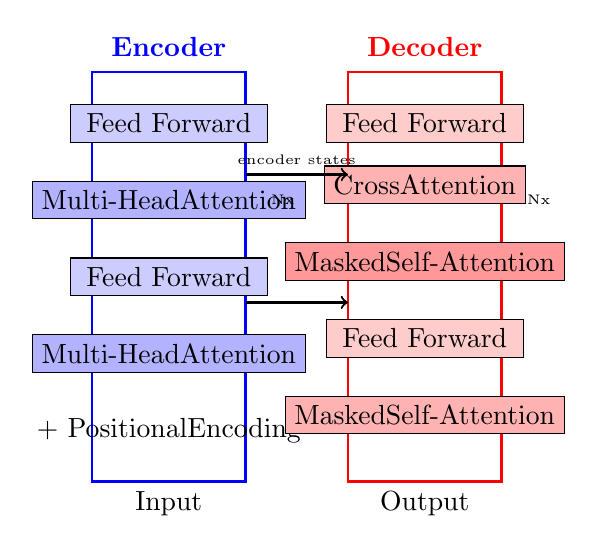
\begin{tikzpicture}[scale=0.65]
    % Encoder
    \draw[thick,blue] (0, 0) rectangle (3, 8);
    \node[blue] at (1.5, 8.5) {\textbf{Encoder}};

    % Encoder components
    \node[rectangle,draw,fill=blue!20,minimum width=2.5cm] at (1.5, 7) {Feed Forward};
    \node[rectangle,draw,fill=blue!30,minimum width=2.5cm] at (1.5, 5.5) {Multi-Head\\Attention};
    \node[rectangle,draw,fill=blue!20,minimum width=2.5cm] at (1.5, 4) {Feed Forward};
    \node[rectangle,draw,fill=blue!30,minimum width=2.5cm] at (1.5, 2.5) {Multi-Head\\Attention};
    \node at (1.5, 1) {+ Positional\\Encoding};
    \node[below] at (1.5, 0) {Input};

    % Decoder
    \draw[thick,red] (5, 0) rectangle (8, 8);
    \node[red] at (6.5, 8.5) {\textbf{Decoder}};

    % Decoder components
    \node[rectangle,draw,fill=red!20,minimum width=2.5cm] at (6.5, 7) {Feed Forward};
    \node[rectangle,draw,fill=red!30,minimum width=2.5cm] at (6.5, 5.8) {Cross\\Attention};
    \node[rectangle,draw,fill=red!40,minimum width=2.5cm] at (6.5, 4.3) {Masked\\Self-Attention};
    \node[rectangle,draw,fill=red!20,minimum width=2.5cm] at (6.5, 2.8) {Feed Forward};
    \node[rectangle,draw,fill=red!30,minimum width=2.5cm] at (6.5, 1.3) {Masked\\Self-Attention};
    \node[below] at (6.5, 0) {Output};

    % Arrows
    \draw[->, thick] (3, 6) -- (5, 6) node[midway,above] {\tiny encoder states};
    \draw[->, thick] (3, 3.5) -- (5, 3.5);

    % Stack indicators
    \node[right=0.2cm of {(3,5.5)}] {\tiny Nx};
    \node[right=0.2cm of {(8,5.5)}] {\tiny Nx};
\end{tikzpicture}
\end{center}

\textbf{Key Components:}
\begin{itemize}\setlength{\itemsep}{0pt}
    \item \textbf{Multi-Head Self-Attention}: Relate all positions to each other
    \item \textbf{Feed-Forward Networks}: Transform representations
    \item \textbf{Residual Connections \& Layer Norm}: Training stability (not shown)
    \item \textbf{Positional Encoding}: Inject position information
\end{itemize}
\end{frame}

% ============================================================
% SELF ATTENTION
% ============================================================
\begin{frame}[shrink=5]{Self-Attention: The Core Mechanism 🎯}
\textbf{Key idea: Each word attends to all other words in the sequence}

\vspace{1em}

\textbf{Three learned projections:}
\begin{itemize}\setlength{\itemsep}{0pt}
    \item \textbf{Query (Q)}: What am I looking for?
    \item \textbf{Key (K)}: What do I contain?
    \item \textbf{Value (V)}: What information do I have?
\end{itemize}

\vspace{1em}

\textbf{Computation:}
\begin{align*}
Q = XW_Q, \quad K = XW_K, \quad V = XW_V
\end{align*}
\begin{align*}
\text{Attention}(Q, K, V) = \text{softmax}\left(\frac{QK^T}{\sqrt{d_k}}\right)V
\end{align*}

\vspace{1em}

\begin{center}
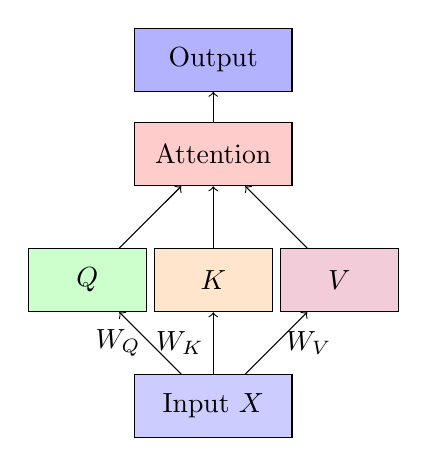
\begin{tikzpicture}[scale=0.8]
    \node[rectangle,draw,fill=blue!20,minimum width=2cm,minimum height=0.8cm] (x) at (0, 0) {Input $X$};

    \node[rectangle,draw,fill=green!20,minimum width=1.5cm,minimum height=0.8cm] (q) at (-2, 2) {$Q$};
    \node[rectangle,draw,fill=orange!20,minimum width=1.5cm,minimum height=0.8cm] (k) at (0, 2) {$K$};
    \node[rectangle,draw,fill=purple!20,minimum width=1.5cm,minimum height=0.8cm] (v) at (2, 2) {$V$};

    \draw[->] (x) -- (q) node[midway,left] {$W_Q$};
    \draw[->] (x) -- (k) node[midway,left] {$W_K$};
    \draw[->] (x) -- (v) node[midway,right] {$W_V$};

    \node[rectangle,draw,fill=red!20,minimum width=2cm,minimum height=0.8cm] (attn) at (0, 4) {Attention};
    \draw[->] (q) -- (attn);
    \draw[->] (k) -- (attn);
    \draw[->] (v) -- (attn);

    \node[rectangle,draw,fill=blue!30,minimum width=2cm,minimum height=0.8cm] (out) at (0, 5.5) {Output};
    \draw[->] (attn) -- (out);
\end{tikzpicture}
\end{center}
\end{frame}

% ============================================================
% QKV INTUITION
% ============================================================
\begin{frame}[shrink=10]{Understanding Query, Key, Value 🔑}
\small
\textbf{Analogy: Database lookup or information retrieval}

\vspace{1em}

\begin{columns}[T]
\begin{column}{0.48\textwidth}
\textbf{Information Retrieval:}
\begin{itemize}\setlength{\itemsep}{0pt}
    \item \textbf{Query}: Your search query
    \item \textbf{Key}: Document titles/keywords
    \item \textbf{Value}: Document contents
\end{itemize}

\vspace{0.5em}

\textbf{Process:}
\begin{enumerate}\setlength{\itemsep}{0pt}
    \item Compare query to all keys
    \item Get similarity scores
    \item Weight values by scores
    \item Return weighted combination
\end{enumerate}
\end{column}

\begin{column}{0.48\textwidth}
\textbf{Self-Attention:}
\begin{itemize}\setlength{\itemsep}{0pt}
    \item \textbf{Query}: What token $i$ is looking for
    \item \textbf{Key}: What token $j$ offers
    \item \textbf{Value}: Information from token $j$
\end{itemize}

\vspace{0.5em}

\textbf{Process:}
\begin{enumerate}\setlength{\itemsep}{0pt}
    \item Compare $Q_i$ to all $K_j$
    \item Get attention scores
    \item Weight all $V_j$ by scores
    \item Return new representation for $i$
\end{enumerate}
\end{column}
\end{columns}

\vspace{1em}

\begin{block}{Key Insight}
Each token simultaneously acts as:
\begin{itemize}\setlength{\itemsep}{0pt}
    \item A query (what it needs from other tokens)
    \item A key (how it should be retrieved)
    \item A value (what information it provides)
\end{itemize}
\end{block}
\end{frame}

% ============================================================
% SCALED DOT PRODUCT
% ============================================================
\begin{frame}[shrink=10]{Scaled Dot-Product Attention 📐}
\textbf{Step-by-step computation:}

\vspace{1em}

\begin{align*}
\text{Attention}(Q, K, V) = \text{softmax}\left(\frac{QK^T}{\sqrt{d_k}}\right)V
\end{align*}

\vspace{1em}

\begin{enumerate}\setlength{\itemsep}{0pt}
    \item \textbf{Compute scores}: $S = QK^T$
    \begin{itemize}\setlength{\itemsep}{0pt}
        \item Matrix multiplication: $[n \times d_k] \times [d_k \times n] = [n \times n]$
        \item Each element $S_{ij}$ = similarity between token $i$ and $j$
    \end{itemize}

    \item \textbf{Scale}: $S' = S / \sqrt{d_k}$
    \begin{itemize}\setlength{\itemsep}{0pt}
        \item Prevents gradients from becoming too small
        \item When $d_k$ is large, dot products grow large
        \item Scaling keeps softmax gradients stable
    \end{itemize}

    \item \textbf{Softmax}: $A = \text{softmax}(S')$
    \begin{itemize}\setlength{\itemsep}{0pt}
        \item Convert to probability distribution (rows sum to 1)
        \item Each row = attention distribution for one token
    \end{itemize}

    \item \textbf{Weighted sum}: $\text{Output} = AV$
    \begin{itemize}\setlength{\itemsep}{0pt}
        \item $[n \times n] \times [n \times d_v] = [n \times d_v]$
        \item Each output is a weighted combination of all values
    \end{itemize}
\end{enumerate}
\end{frame}

% ============================================================
% SELF ATTENTION EXAMPLE
% ============================================================
\begin{frame}[shrink=5]{Self-Attention Example 📝}
\textbf{Sentence: "The animal didn't cross the street because it was too tired"}

\vspace{1em}

\textbf{Question: What does "it" refer to?}

\vspace{1em}

\begin{center}
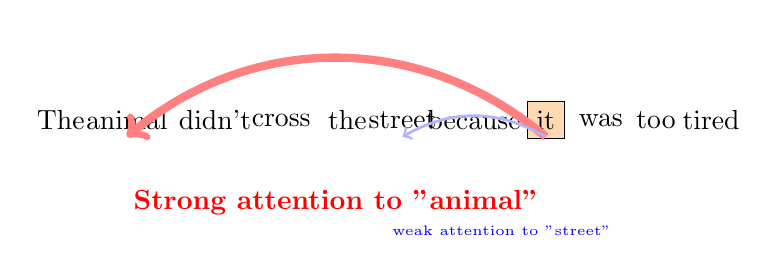
\begin{tikzpicture}[scale=0.7]
    % Words
    \node at (0, 2) {The};
    \node at (1.2, 2) {animal};
    \node at (2.8, 2) {didn't};
    \node at (4, 2) {cross};
    \node at (5.2, 2) {the};
    \node at (6.2, 2) {street};
    \node at (7.5, 2) {because};
    \node[rectangle,draw,fill=orange!30] at (8.8, 2) {it};
    \node at (9.8, 2) {was};
    \node at (10.8, 2) {too};
    \node at (11.8, 2) {tired};

    % Attention from "it"
    \draw[->, thick, line width=3pt, red!50] (8.8, 1.7) to[bend right=40] (1.2, 1.7);
    \node[red] at (5, 0.5) {\textbf{Strong attention to "animal"}};

    \draw[->, thick, line width=1pt, blue!30] (8.8, 1.7) to[bend right=30] (6.2, 1.7);
    \node[blue] at (8, 0) {\tiny weak attention to "street"};
\end{tikzpicture}
\end{center}

\vspace{1em}

\textbf{Self-attention allows the model to:}
\begin{itemize}\setlength{\itemsep}{0pt}
    \item Resolve pronouns
    \item Understand long-range dependencies
    \item Capture syntactic and semantic relationships
    \item Do this in parallel for all positions!
\end{itemize}
\end{frame}

% ============================================================
% ATTENTION MATRIX
% ============================================================
\begin{frame}{Visualizing the Attention Matrix 🔍}
\textbf{For sentence: "The cat sat on the mat"}

\vspace{1em}

\begin{center}
\small
\begin{tabular}{c|cccccc}
\textbf{To $\rightarrow$} & The & cat & sat & on & the & mat \\
\textbf{From $\downarrow$} & & & & & & \\
\hline
The & 0.3 & 0.4 & 0.1 & 0.1 & 0.05 & 0.05 \\
cat & 0.1 & \cellcolor{orange!80}0.5 & 0.2 & 0.1 & 0.05 & 0.05 \\
sat & 0.05 & 0.3 & \cellcolor{orange!80}0.4 & 0.15 & 0.05 & 0.05 \\
on & 0.05 & 0.1 & 0.2 & 0.3 & 0.1 & 0.25 \\
the & 0.05 & 0.05 & 0.05 & 0.1 & 0.3 & 0.45 \\
mat & 0.05 & 0.05 & 0.1 & 0.2 & 0.2 & \cellcolor{orange!80}0.4 \\
\end{tabular}
\end{center}

\vspace{1em}

\textbf{Observations:}
\begin{itemize}\setlength{\itemsep}{0pt}
    \item Each row sums to 1.0 (probability distribution)
    \item Diagonal elements often high (self-attention)
    \item "cat" attends to itself and "The" (determiner-noun relationship)
    \item "mat" attends to "the" (determiner) and "on" (preposition)
    \item Captures syntactic and semantic structure automatically!
\end{itemize}
\end{frame}

% ============================================================
% MULTI HEAD ATTENTION
% ============================================================
\begin{frame}[shrink=5]{Multi-Head Attention 🎭}
\textbf{Why use multiple attention heads?}

\vspace{1em}

\begin{columns}[T]
\begin{column}{0.48\textwidth}
\textbf{Intuition:}
\begin{itemize}\setlength{\itemsep}{0pt}
    \item Different heads learn different relationships
    \item Head 1: Syntactic relationships
    \item Head 2: Semantic relationships
    \item Head 3: Positional patterns
    \item Etc.
\end{itemize}

\vspace{1em}

\textbf{Formula:}
\begin{align*}
\text{MultiHead}(Q,K,V) &= \text{Concat}(h_1, ..., h_H)W_O \\
h_i &= \text{Attention}(QW_i^Q, KW_i^K, VW_i^V)
\end{align*}
\end{column}

\begin{column}{0.48\textwidth}
\begin{center}
\begin{tikzpicture}[scale=0.65]
    \node[rectangle,draw,fill=blue!20] (input) at (2, 0) {Input};

    % Multiple heads
    \foreach \x/\name in {0/Head 1, 1.5/Head 2, 3/Head 3, 4.5/Head H} {
        \node[rectangle,draw,fill=green!20,minimum width=1cm,minimum height=0.6cm] (h\x) at (\x, 2) {\tiny\name};
        \draw[->] (input) -- (h\x);
    }

    \node at (5.5, 2) {\tiny ...};

    % Concatenate
    \node[rectangle,draw,fill=orange!20,minimum width=5cm,minimum height=0.8cm] (concat) at (2, 4) {Concatenate};
    \foreach \x in {0, 1.5, 3, 4.5} {
        \draw[->] (h\x) -- (concat);
    }

    % Linear
    \node[rectangle,draw,fill=purple!20,minimum width=3cm,minimum height=0.8cm] (linear) at (2, 5.5) {Linear ($W_O$)};
    \draw[->] (concat) -- (linear);

    % Output
    \node[rectangle,draw,fill=red!20] (output) at (2, 7) {Output};
    \draw[->] (linear) -- (output);
\end{tikzpicture}
\end{center}

\vspace{0.5em}
\textbf{Typical:} 8-16 heads in practice
\end{column}
\end{columns}

\vspace{0.5em}
\textit{BERT-base: 12 heads, BERT-large: 16 heads, GPT-3: 96 heads!}
\end{frame}

% ============================================================
% WHY MULTI HEAD
% ============================================================
\begin{frame}[shrink=10]{Why Multiple Heads? 🤔}
\small
\textbf{Example: Different heads learn different patterns}

\vspace{1em}

\textbf{Sentence: "The cat sat on the mat"}

\vspace{0.5em}

\begin{columns}[T]
\begin{column}{0.48\textwidth}
\textbf{Head 1: Syntactic Dependencies}
\begin{itemize}\setlength{\itemsep}{0pt}
    \item "cat" → "The" (noun-determiner)
    \item "sat" → "cat" (verb-subject)
    \item "mat" → "the" (noun-determiner)
    \item Learns grammar structure
\end{itemize}

\vspace{0.5em}

\textbf{Head 2: Semantic Relations}
\begin{itemize}\setlength{\itemsep}{0pt}
    \item "sat" → "mat" (action-location)
    \item "cat" → "mat" (agent-location)
    \item Learns meaning relationships
\end{itemize}
\end{column}

\begin{column}{0.48\textwidth}
\textbf{Head 3: Local Context}
\begin{itemize}\setlength{\itemsep}{0pt}
    \item Each word → neighbors
    \item Short-range dependencies
    \item N-gram like patterns
\end{itemize}

\vspace{0.5em}

\textbf{Head 4: Long-Range}
\begin{itemize}\setlength{\itemsep}{0pt}
    \item Distant word relationships
    \item Document-level context
    \item Coreference resolution
\end{itemize}
\end{column}
\end{columns}

\vspace{1em}

\begin{block}{Ensemble Effect}
Multiple heads provide a richer, more diverse representation by attending to different aspects of the input simultaneously!
\end{block}
\end{frame}

% ============================================================
% TYPES OF ATTENTION
% ============================================================
\begin{frame}[shrink=10]{Three Types of Attention 🔍}
\begin{enumerate}\setlength{\itemsep}{0pt}
    \item \textbf{Self-Attention (Encoder)}
    \begin{itemize}\setlength{\itemsep}{0pt}
        \item Each position attends to all positions in same sequence
        \item Bidirectional: can see past and future
        \item Used in: BERT, encoder-only models
    \end{itemize}

    \vspace{0.5em}

    \item \textbf{Masked Self-Attention (Decoder)}
    \begin{itemize}\setlength{\itemsep}{0pt}
        \item Each position attends only to previous positions
        \item Prevents "looking into the future"
        \item Used in: GPT, decoder-only models
    \end{itemize}

    \vspace{0.5em}

    \item \textbf{Cross-Attention (Encoder-Decoder)}
    \begin{itemize}\setlength{\itemsep}{0pt}
        \item Decoder attends to encoder outputs
        \item Queries from decoder, Keys/Values from encoder
        \item Used in: T5, BART, machine translation
    \end{itemize}
\end{enumerate}

\vspace{1em}

\begin{center}
\begin{tabular}{lcc}
\toprule
\textbf{Type} & \textbf{Q from} & \textbf{K, V from} \\
\midrule
Self-Attention & Sequence & Same sequence \\
Masked Self-Attention & Sequence & Same sequence (past only) \\
Cross-Attention & Decoder & Encoder \\
\bottomrule
\end{tabular}
\end{center}
\end{frame}

% ============================================================
% MASKED ATTENTION
% ============================================================
\begin{frame}{Masked Self-Attention 🎭}
\textbf{Preventing the model from "cheating" during generation}

\vspace{1em}

\textbf{Problem:} During training, we have the full target sequence. Without masking, the model could "peek" at future tokens!

\vspace{0.5em}

\textbf{Solution:} Mask out future positions by setting attention scores to $-\infty$ before softmax.

\vspace{1em}

\begin{center}
\small
\textbf{Attention scores before masking:}

\begin{tabular}{c|cccc}
 & $t_1$ & $t_2$ & $t_3$ & $t_4$ \\
\hline
$t_1$ & 0.5 & \cellcolor{red!30}-inf & \cellcolor{red!30}-inf & \cellcolor{red!30}-inf \\
$t_2$ & 0.3 & 0.4 & \cellcolor{red!30}-inf & \cellcolor{red!30}-inf \\
$t_3$ & 0.2 & 0.3 & 0.4 & \cellcolor{red!30}-inf \\
$t_4$ & 0.15 & 0.25 & 0.3 & 0.35 \\
\end{tabular}

\vspace{0.5em}

\textbf{After softmax:} Future positions have weight 0
\end{center}

\vspace{1em}

\textbf{Result:} Token at position $t$ can only attend to positions $\leq t$
\begin{itemize}\setlength{\itemsep}{0pt}
    \item Maintains autoregressive property
    \item Enables parallel training while preserving causality
\end{itemize}
\end{frame}

% ============================================================
% CROSS ATTENTION
% ============================================================
\begin{frame}[shrink=5]{Cross-Attention 🔗}
\textbf{Connecting encoder and decoder in seq2seq models}

\vspace{1em}

\begin{center}
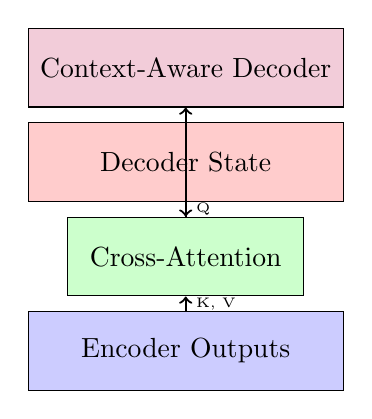
\begin{tikzpicture}[scale=0.8]
    % Encoder outputs
    \node[rectangle,draw,fill=blue!20,minimum width=4cm,minimum height=1cm] (enc) at (0, 0) {Encoder Outputs};
    \node[above=0.1cm of enc] {\small (Keys \& Values)};

    % Decoder state
    \node[rectangle,draw,fill=red!20,minimum width=4cm,minimum height=1cm] (dec) at (0, 3) {Decoder State};
    \node[above=0.1cm of dec] {\small (Queries)};

    % Cross attention
    \node[rectangle,draw,fill=green!20,minimum width=3cm,minimum height=1cm] (cross) at (0, 1.5) {Cross-Attention};

    % Arrows
    \draw[->, thick] (enc) -- (cross) node[midway,right] {\tiny K, V};
    \draw[->, thick] (dec) -- (cross) node[midway,right] {\tiny Q};

    % Output
    \node[rectangle,draw,fill=purple!20,minimum width=4cm,minimum height=1cm] (out) at (0, 4.5) {Context-Aware Decoder};
    \draw[->, thick] (cross) -- (out);
\end{tikzpicture}
\end{center}

\vspace{1em}

\textbf{Key Properties:}
\begin{itemize}\setlength{\itemsep}{0pt}
    \item \textbf{Q} comes from decoder (what decoder needs)
    \item \textbf{K, V} come from encoder (what input provides)
    \item Allows decoder to "look at" relevant parts of input
    \item Similar to the original attention mechanism from Lecture 12!
\end{itemize}

\vspace{0.5em}

\textbf{Used in:} Machine translation, summarization, any encoder-decoder task
\end{frame}

% ============================================================
% CODE EXAMPLE
% ============================================================
\begin{frame}[fragile]{Implementing Self-Attention in PyTorch 💻}
\textbf{Scaled dot-product attention}

\begin{lstlisting}[language=Python]
import torch
import torch.nn as nn
import torch.nn.functional as F
import math

class SelfAttention(nn.Module):
    def __init__(self, embed_dim):
        super().__init__()
        self.embed_dim = embed_dim
        self.W_q = nn.Linear(embed_dim, embed_dim)
        self.W_k = nn.Linear(embed_dim, embed_dim)
        self.W_v = nn.Linear(embed_dim, embed_dim)

    def forward(self, x, mask=None):
        # x: [batch, seq_len, embed_dim]
        Q = self.W_q(x)  # [batch, seq_len, embed_dim]
        K = self.W_k(x)
        V = self.W_v(x)

        # Compute attention scores
        scores = torch.matmul(Q, K.transpose(-2, -1))  # [batch, seq_len, seq_len]
        scores = scores / math.sqrt(self.embed_dim)

        # Apply mask if provided (for decoder)
        if mask is not None:
            scores = scores.masked_fill(mask == 0, -1e9)

        # Softmax to get attention weights
        attn_weights = F.softmax(scores, dim=-1)

        # Apply attention to values
        output = torch.matmul(attn_weights, V)  # [batch, seq_len, embed_dim]

        return output, attn_weights
\end{lstlisting}
\end{frame}

% ============================================================
% COMPLEXITY
% ============================================================
\begin{frame}[shrink=10]{Computational Complexity ⚙️}
\textbf{Understanding the cost of self-attention}

\vspace{1em}

\begin{center}
\begin{tabular}{lcc}
\toprule
\textbf{Operation} & \textbf{Time Complexity} & \textbf{Space Complexity} \\
\midrule
RNN/LSTM & $O(n \cdot d^2)$ & $O(d)$ \\
Self-Attention & $O(n^2 \cdot d)$ & $O(n^2)$ \\
Feed-Forward & $O(n \cdot d^2)$ & $O(d)$ \\
\bottomrule
\end{tabular}

\vspace{0.5em}
\small
where $n$ = sequence length, $d$ = embedding dimension
\end{center}

\vspace{1em}

\textbf{Trade-offs:}
\begin{columns}[T]
\begin{column}{0.48\textwidth}
\textbf{Pros of Self-Attention:}
\begin{itemize}\setlength{\itemsep}{0pt}
    \item Parallelizable (all positions at once)
    \item Direct connections between all tokens
    \item No vanishing gradients
\end{itemize}
\end{column}

\begin{column}{0.48\textwidth}
\textbf{Cons of Self-Attention:}
\begin{itemize}\setlength{\itemsep}{0pt}
    \item Quadratic in sequence length
    \item Memory intensive for long sequences
    \item Limits context window size
\end{itemize}
\end{column}
\end{columns}

\vspace{1em}

\textbf{Typical limits:}
\begin{itemize}\setlength{\itemsep}{0pt}
    \item BERT: 512 tokens
    \item GPT-2: 1024 tokens
    \item GPT-3: 2048 tokens
    \item Modern models: 4096-100k tokens (with optimizations)
\end{itemize}
\end{frame}

% ============================================================
% DISCUSSION
% ============================================================
\begin{frame}[shrink=10]{Discussion Questions 💭}
\begin{enumerate}\setlength{\itemsep}{0pt}
    \item \textbf{Self-Attention vs RNN Attention:}
    \begin{itemize}\setlength{\itemsep}{0pt}
        \item What's the key difference?
        \item Why is self-attention more powerful?
        \item When might RNNs still be useful?
    \end{itemize}

    \vspace{0.5em}

    \item \textbf{Query, Key, Value Framework:}
    \begin{itemize}\setlength{\itemsep}{0pt}
        \item Why three separate projections instead of one?
        \item What if we used $Q = K = V = X$?
        \item How does this relate to information retrieval?
    \end{itemize}

    \vspace{0.5em}

    \item \textbf{Multi-Head Attention:}
    \begin{itemize}\setlength{\itemsep}{0pt}
        \item Why not just use one big attention head?
        \item How many heads is optimal?
        \item Can we interpret what each head learns?
    \end{itemize}

    \vspace{0.5em}

    \item \textbf{Scalability:}
    \begin{itemize}\setlength{\itemsep}{0pt}
        \item $O(n^2)$ is problematic for long documents. Solutions?
        \item Sparse attention? Local attention? Other ideas?
    \end{itemize}
\end{enumerate}
\end{frame}

% ============================================================
% LOOKING AHEAD
% ============================================================
\begin{frame}[shrink=10]{Looking Ahead 🔮}
\textbf{What's Next?}

\vspace{1em}

\textbf{Today we learned:}
\begin{itemize}\setlength{\itemsep}{0pt}
    \item Why transformers replaced RNNs
    \item Self-attention mechanism (Q, K, V)
    \item Multi-head attention
    \item Three types of attention (self, masked, cross)
\end{itemize}

\vspace{1em}

\textbf{Next lecture (Lecture 14 - Training Transformers):}
\begin{itemize}\setlength{\itemsep}{0pt}
    \item \alert{Positional Encoding}: How to inject position information
    \item \alert{Feed-Forward Networks}: The other key component
    \item \alert{Layer Normalization \& Residuals}: Training stability
    \item \alert{FlashAttention}: Making transformers faster
    \item \alert{Three Architectures}: Encoder, Decoder, Encoder-Decoder
    \item \alert{Practical Tips}: Training and using transformers
\end{itemize}

\vspace{1em}

\begin{center}
\Large
\textbf{We're building up to BERT and GPT! 🚀}
\end{center}
\end{frame}

% ============================================================
% SUMMARY
% ============================================================
\begin{frame}[shrink=10]{Summary 🎯}
\textbf{Key Takeaways:}

\vspace{1em}

\begin{enumerate}\setlength{\itemsep}{0pt}
    \item \textbf{Transformer Revolution}
    \begin{itemize}\setlength{\itemsep}{0pt}
        \item Pure attention, no recurrence
        \item Parallel processing, faster training
    \end{itemize}

    \item \textbf{Self-Attention Mechanism}
    \begin{itemize}\setlength{\itemsep}{0pt}
        \item Query, Key, Value framework
        \item Each token attends to all others
        \item Scaled dot-product: $\text{softmax}(QK^T/\sqrt{d_k})V$
    \end{itemize}

    \item \textbf{Multi-Head Attention}
    \begin{itemize}\setlength{\itemsep}{0pt}
        \item Multiple heads learn diverse relationships
        \item Concatenate and project back
        \item Richer representations
    \end{itemize}

    \item \textbf{Three Attention Types}
    \begin{itemize}\setlength{\itemsep}{0pt}
        \item Self (encoder), Masked (decoder), Cross (encoder-decoder)
        \item Different uses for different architectures
    \end{itemize}
\end{enumerate}

\vspace{0.5em}
\textbf{Self-attention is the foundation of modern NLP!}
\end{frame}

% ============================================================
% REFERENCES
% ============================================================
\begin{frame}[shrink=10]{References 📚}
\textbf{Essential Papers:}

\vspace{0.5em}

\begin{itemize}\setlength{\itemsep}{0pt}
    \item \textbf{Vaswani et al. (2017)} - "Attention Is All You Need"
    \begin{itemize}\setlength{\itemsep}{0pt}
        \item The original Transformer paper
        \item Introduced self-attention, multi-head attention
        \item Foundation of modern NLP
    \end{itemize}

    \vspace{0.3em}

    \item \textbf{Bahdanau et al. (2015)} - "Neural Machine Translation by Jointly Learning to Align and Translate"
    \begin{itemize}\setlength{\itemsep}{0pt}
        \item Original attention mechanism (for comparison)
    \end{itemize}
\end{itemize}

\vspace{0.5em}

\textbf{Tutorials and Resources:}
\begin{itemize}\setlength{\itemsep}{0pt}
    \item \textbf{The Illustrated Transformer} by Jay Alammar
    \begin{itemize}\setlength{\itemsep}{0pt}
        \item \url{https://jalammar.github.io/illustrated-transformer/}
        \item Visual step-by-step explanation
    \end{itemize}

    \vspace{0.3em}

    \item \textbf{Annotated Transformer} by Harvard NLP
    \begin{itemize}\setlength{\itemsep}{0pt}
        \item \url{https://nlp.seas.harvard.edu/annotated-transformer/}
        \item Line-by-line implementation
    \end{itemize}

    \vspace{0.3em}

    \item \textbf{HuggingFace Course} - Chapter 1.4
    \begin{itemize}\setlength{\itemsep}{0pt}
        \item How Transformers work
    \end{itemize}
\end{itemize}
\end{frame}

% ============================================================
% QUESTIONS
% ============================================================
\begin{frame}{Questions? 🙋}
\begin{center}
\LARGE
\textbf{Discussion Time}
\end{center}

\vspace{1em}

\textbf{Topics for discussion:}
\begin{itemize}\setlength{\itemsep}{0pt}
    \item Self-attention mechanism
    \item Query, Key, Value intuition
    \item Multi-head attention
    \item Masked vs. unmasked attention
    \item Implementation questions
\end{itemize}

\vspace{1em}

\begin{center}
\Large
Thank you! 🙏

\vspace{1em}

Next: Training Transformers!
\end{center}
\end{frame}

\end{document}
